% Phys 39 Module 4 -- A2: TEC Heating And Cooling Analysis
% Build:  cd a2 && latexmk -pdf A2.tex   (or: pdflatex A2.tex)
% Rename the PDF to A2_Lastname_Lastname.pdf before uploading to Moodle.
\documentclass[10pt]{article}
\usepackage[margin=0.6in]{geometry}
\usepackage{amsmath,amssymb}
\usepackage[compact,small]{titlesec}
\usepackage{graphicx}
\usepackage{booktabs}
\usepackage[font=small,labelfont=bf]{caption}
\usepackage[T1]{fontenc}
\usepackage{lmodern}
\usepackage{enumitem}
\setlist{nosep,leftmargin=1.2em}
\setlength{\parindent}{0pt}
\setlength{\parskip}{0.35em}

% Fill in the team names.
\newcommand{\teamnames}{Firstname Lastname \& Firstname Lastname}

\newcommand{\Qdot}{\dot Q}
\newcommand{\degC}{\,^\circ\mathrm{C}}

\begin{document}

\begin{center}
  {\large\bfseries A2: TEC Heating and Cooling Analysis}\\[2pt]
  Phys 39, Module 4 \quad\textbullet\quad \teamnames
\end{center}

%-----------------------------------------------------------------------
\section*{1. Part 4: Combined graph and fits}

\begin{figure}[h]
  \centering
  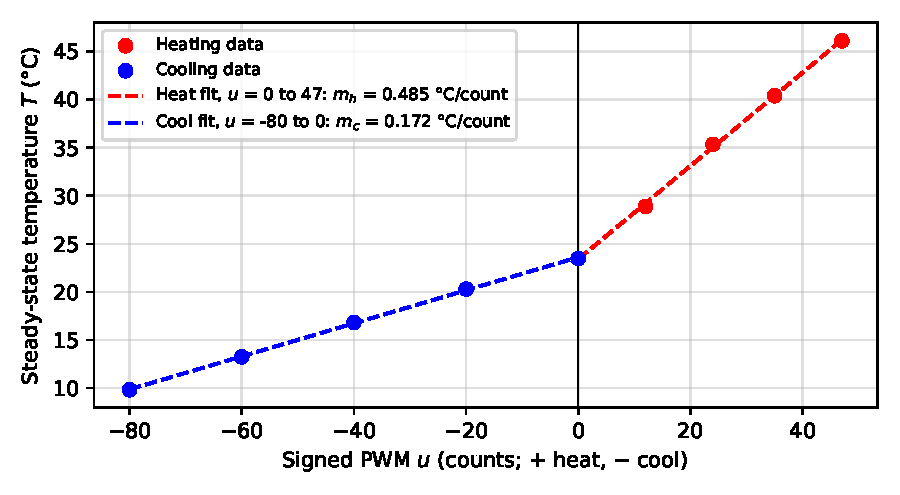
\includegraphics[width=0.66\linewidth]{figures/temp_vs_signed_pwm.pdf}
  \caption{Steady-state temperature versus signed PWM $u$ (positive = heating, red;
  negative = cooling, blue), with a least-squares line for each branch. Heating fit:
  $u = 0$ to $47$; cooling fit: $u = -80$ to $0$. Both branches share the $u = 0$ point
  ($23.48\degC$). Steady state: after each PWM step we waited about three time constants
  ($\tau \lesssim 100$\,s), then recorded the temperature once it stayed within
  $\pm 0.1\degC$ (about the normal measurement noise) for one further minute. Waits were
  370--725\,s.}
\end{figure}

%-----------------------------------------------------------------------
\section*{2. Part 5.1: Measured slopes}

\begin{tabular}{@{}lccc@{}}
  \toprule
  Branch & Fit range (signed PWM) & Duty range $D$ & Slope \\
  \midrule
  Heating & $0$ to $+47$  & $0$--$0.184$ & $m_h = 0.485 \pm 0.007\degC/\text{count}$ \\
  Cooling & $-80$ to $0$ & $0$--$0.314$ & $m_c = 0.172 \pm 0.002\degC/\text{count}$ \\
  \bottomrule
\end{tabular}

\[
r = \frac{m_h}{m_c} = \frac{0.485}{0.172} = 2.82 \pm 0.05 .
\]
(Uncertainties are the standard errors of the fitted slopes.) Neither branch shows visible
curvature: the slopes between neighbouring points are $0.45, 0.54, 0.46, 0.48\degC$/count
(heating) and $0.17, 0.18, 0.17, 0.16\degC$/count (cooling), with no systematic trend. We
therefore fitted one straight line to all five points of each branch, from $0$ to that
direction's maximum useful PWM.

%-----------------------------------------------------------------------
\section*{3. Part 5.2: PWM and the slope-ratio model}

\textbf{Steady-state balance.} At steady state $G(T-T_0) = \Qdot_{\mathrm{TEC}}$.
$\Qdot_{\mathrm{TEC}}$ holds the two current-dependent object-face terms: Peltier transport
(into the object when heating, out of it when cooling) and object-face Joule heating
$\tfrac12 I^2 R_M$ (always into the object). $G(T-T_0)$ is the net passive heat flow out of
the object, including conduction back through the TEC. When heating ($T>T_0$) it flows out;
when cooling ($T<T_0$) it flows in. The individual flows are not zero; their sum is.

\textbf{PWM averages.} In one period $\tau$ the current is $I$ for $D\tau$ and $0$ for
$(1-D)\tau$, so
\[
\langle I\rangle = \frac1\tau\!\left[\int_0^{D\tau}\! I\,dt + \int_{D\tau}^{\tau}\! 0\,dt\right]
= \frac{I\,D\tau}{\tau} = D I,
\qquad
\langle I^2\rangle = \frac1\tau\int_0^{D\tau}\! I^2\,dt = D I^2 .
\]
Because the current is either full or zero, $\langle I^2\rangle = DI^2 \neq \langle
I\rangle^2 = D^2I^2$ for $0<D<1$. Both terms are therefore linear in $D$, and the model
predicts a straight line on each branch with a kink at $u=0$. This matches our graph. With
$\langle I^2\rangle = D^2I^2$ (as for DC), the heating branch would curve upward and the
cooling branch would flatten. This assumes the PWM period ($\approx 2$\,ms) is much shorter
than the thermal time constant, so the block responds only to the averages.

\textbf{Slope ratio.} With signed duty $d = u/255$ and $D = |d|$,
$\Qdot_{\mathrm{TEC}} = d\,\Qdot_P + |d|\,\Qdot_J$.
\begin{align*}
\text{Heating } (d>0,\ |d| = d):&\quad G(T_h - T_0) = d(\Qdot_P + \Qdot_J)
  &&\Rightarrow\quad \frac{dT_h}{dd} = \frac{\Qdot_P + \Qdot_J}{G},\\
\text{Cooling } (d<0,\ |d| = -d):&\quad G(T_c - T_0) = d(\Qdot_P - \Qdot_J)
  &&\Rightarrow\quad \frac{dT_c}{dd} = \frac{\Qdot_P - \Qdot_J}{G}.
\end{align*}
Both slopes are positive when $\Qdot_P > \Qdot_J$, and the heating slope is larger.
Since $m = dT/du = \tfrac{1}{255}\,dT/dd$, the factors $1/255$ and $G$ cancel:
\[
r = \frac{m_h}{m_c} = \frac{\Qdot_P + \Qdot_J}{\Qdot_P - \Qdot_J}.
\]
Let $x = \Qdot_J/\Qdot_P$. Then $r = (1+x)/(1-x)$, so $r - rx = 1 + x$, $r - 1 = x(r+1)$, and
\[
\boxed{\frac{\Qdot_J}{\Qdot_P} = \frac{r-1}{r+1}}
= \frac{2.82 - 1}{2.82 + 1} = 0.48 \pm 0.01 .
\]
(Check: $r = 2$ gives $1/3$.) At our on-state current, the object-face Joule heat is about
half of the Peltier heat pumping.

%-----------------------------------------------------------------------
\section*{4. Part 5.3: Laird data-sheet calculation}

Source: Laird CP14-127-045-L2-W4.5 data sheet (Rev.\ 00, 06-01-2022), p.\,3,
\emph{Specifications} table, hot-side temperature $T_h = 27.0\degC$ column.

\begin{tabular}{@{}lll@{}}
  \toprule
  Quantity & Value & Meaning and operating condition ($T_h = 27\degC$) \\
  \midrule
  $R_M$ & $1.50\ \Omega$ & Electrical resistance of the module. \\
  $I_{\max}$ & $8.6$\,A & Current that produces $\Delta T_{\max}$ with no heat load ($Q_c = 0$). \\
  $Q_{c,\max}$ & $71.3$\,W & Largest heat pumped from the cold side, at $I = I_{\max}$ and $\Delta T = 0$. \\
  $\Delta T_{\max}$ & $70.5\degC$ & Largest hot-to-cold temperature difference, at $I = I_{\max}$ and $Q_c = 0$. \\
  \bottomrule
\end{tabular}

At $\Delta T = 0$ the conduction term is zero. Half of the Joule heat goes to the object face:
\[
\Qdot_{J,\max} = \tfrac12 I_{\max}^2 R_M = \tfrac12\,(8.6\,\mathrm{A})^2(1.50\,\Omega) = 55.5\ \mathrm{W},
\qquad
\Qdot_{P,\max} = Q_{c,\max} + \Qdot_{J,\max} = 71.3 + 55.5 = 126.8\ \mathrm{W},
\]
\[
r_{\mathrm{Laird},\max} = \frac{\Qdot_{P,\max} + \Qdot_{J,\max}}{\Qdot_{P,\max} - \Qdot_{J,\max}}
= \frac{126.8 + 55.5}{126.8 - 55.5} = \frac{182.3}{71.3} = 2.56 .
\]
At $I_{\max}$ this corresponds to $\Qdot_J/\Qdot_P = 55.5/126.8 = 0.44$.

%-----------------------------------------------------------------------
\section*{5. Part 5.4: Compare the ratios}

Measured: $r = 2.82$ ($\Qdot_J/\Qdot_P = 0.48$). Laird at $I_{\max}$: $r = 2.56$ (0.44).
The measured ratio is about 10\,\% higher, which is similar but not equal. Exact agreement
is not expected:
\begin{itemize}
  \item \textbf{$D = 1$ does not mean $I = I_{\max}$.} Full duty only keeps the H-bridge on.
  The on-state current is set by the 12\,V supply, the H-bridge and wiring drops, $R_M$, and
  the TEC's Seebeck back-voltage. That gives at most $12\,\mathrm{V}/1.50\,\Omega \approx 8$\,A
  and in practice less, below $I_{\max} = 8.6$\,A. The 10\,A supply limit is not reached.
  \item \textbf{The Joule fraction scales with current:}
  $\Qdot_J/\Qdot_P = \tfrac12 I^2R_M/(S_M T_o I) \propto I$. A lower current alone would make
  $r$ \emph{smaller} than 2.56, so the excess comes from the effects below.
  \item \textbf{Peltier term $\propto T_o$ (kelvin).} The object face averages $\approx 308$\,K
  on the heating branch and $\approx 290$\,K on the cooling branch, so Peltier pumping is
  relatively stronger when heating. This raises $r$.
  \item \textbf{Finite $\Delta T$, PWM rather than DC, changing properties.} The data sheet is
  for steady DC at $\Delta T = 0$. Our object face spans 10--46\,\textdegree C, which changes
  TEC conduction and the back-voltage. $R_M$ itself rises from 1.50 to 1.68\,$\Omega$ between
  27 and $50\degC$ (same table), and $S_M$ and $K_M$ also vary.
  \item \textbf{Passive paths and fitting.} If the leaks are not equal above and below room
  temperature, $G$ does not cancel exactly. One straight line per branch also averages over
  any slight curvature.
\end{itemize}

%-----------------------------------------------------------------------
\section*{6. Part 5.4: Passive conduction}

When the object is hotter than its surroundings (heating), passive heat flows \emph{out of}
the object; when it is colder (cooling), passive heat flows \emph{into} it. Either way it
pulls the temperature back toward $T_0$, so it opposes both heating and cooling.
Approximately symmetric conduction enters both branches through the same $G$. It reduces both
slopes by the same factor $1/G$, which cancels from $r$. Without Joule heating the two
branches would be $\pm\Qdot_P/G$, equal in magnitude. The unequal slopes come from Joule
heating, which keeps its sign when the current reverses: it adds to Peltier heating and
subtracts from Peltier cooling.

\end{document}
